% Created by tikzDevice version 0.10.1 on 2017-02-08 13:21:36
% !TEX encoding = UTF-8 Unicode
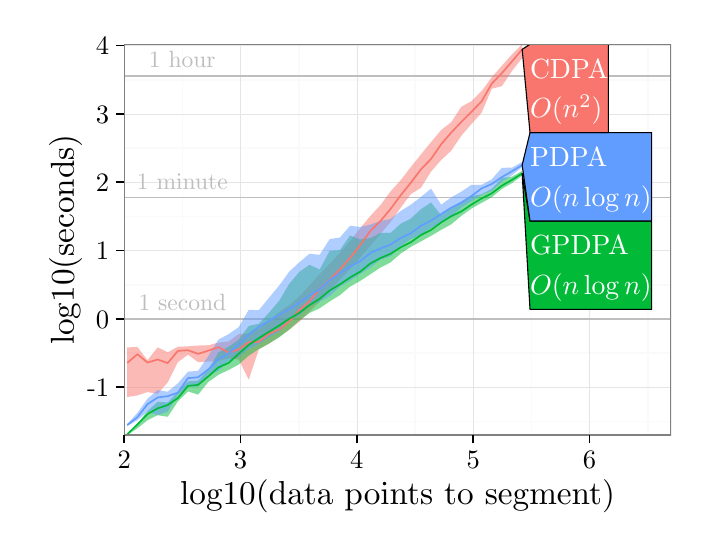
\begin{tikzpicture}[x=1pt,y=1pt]
\definecolor{fillColor}{RGB}{255,255,255}
\path[use as bounding box,fill=fillColor,fill opacity=0.00] (0,0) rectangle (238.49,180.67);
\begin{scope}
\path[clip] (  0.00,  0.00) rectangle (238.49,180.67);
\definecolor{drawColor}{RGB}{255,255,255}
\definecolor{fillColor}{RGB}{255,255,255}

\path[draw=drawColor,line width= 0.6pt,line join=round,line cap=round,fill=fillColor] (  0.00,  0.00) rectangle (238.49,180.68);
\end{scope}
\begin{scope}
\path[clip] ( 34.86, 33.48) rectangle (232.49,174.67);
\definecolor{fillColor}{RGB}{255,255,255}

\path[fill=fillColor] ( 34.86, 33.48) rectangle (232.49,174.67);
\definecolor{drawColor}{gray}{0.98}

\path[draw=drawColor,line width= 0.6pt,line join=round] ( 34.86, 38.39) --
	(232.49, 38.39);

\path[draw=drawColor,line width= 0.6pt,line join=round] ( 34.86, 63.08) --
	(232.49, 63.08);

\path[draw=drawColor,line width= 0.6pt,line join=round] ( 34.86, 87.77) --
	(232.49, 87.77);

\path[draw=drawColor,line width= 0.6pt,line join=round] ( 34.86,112.46) --
	(232.49,112.46);

\path[draw=drawColor,line width= 0.6pt,line join=round] ( 34.86,137.15) --
	(232.49,137.15);

\path[draw=drawColor,line width= 0.6pt,line join=round] ( 34.86,161.84) --
	(232.49,161.84);

\path[draw=drawColor,line width= 0.6pt,line join=round] ( 55.89, 33.48) --
	( 55.89,174.67);

\path[draw=drawColor,line width= 0.6pt,line join=round] ( 97.94, 33.48) --
	( 97.94,174.67);

\path[draw=drawColor,line width= 0.6pt,line join=round] (139.98, 33.48) --
	(139.98,174.67);

\path[draw=drawColor,line width= 0.6pt,line join=round] (182.03, 33.48) --
	(182.03,174.67);

\path[draw=drawColor,line width= 0.6pt,line join=round] (224.08, 33.48) --
	(224.08,174.67);
\definecolor{drawColor}{gray}{0.90}

\path[draw=drawColor,line width= 0.2pt,line join=round] ( 34.86, 50.73) --
	(232.49, 50.73);

\path[draw=drawColor,line width= 0.2pt,line join=round] ( 34.86, 75.42) --
	(232.49, 75.42);

\path[draw=drawColor,line width= 0.2pt,line join=round] ( 34.86,100.12) --
	(232.49,100.12);

\path[draw=drawColor,line width= 0.2pt,line join=round] ( 34.86,124.81) --
	(232.49,124.81);

\path[draw=drawColor,line width= 0.2pt,line join=round] ( 34.86,149.50) --
	(232.49,149.50);

\path[draw=drawColor,line width= 0.2pt,line join=round] ( 34.86,174.19) --
	(232.49,174.19);

\path[draw=drawColor,line width= 0.2pt,line join=round] ( 34.86, 33.48) --
	( 34.86,174.67);

\path[draw=drawColor,line width= 0.2pt,line join=round] ( 76.91, 33.48) --
	( 76.91,174.67);

\path[draw=drawColor,line width= 0.2pt,line join=round] (118.96, 33.48) --
	(118.96,174.67);

\path[draw=drawColor,line width= 0.2pt,line join=round] (161.01, 33.48) --
	(161.01,174.67);

\path[draw=drawColor,line width= 0.2pt,line join=round] (203.06, 33.48) --
	(203.06,174.67);
\definecolor{drawColor}{RGB}{190,190,190}

\path[draw=drawColor,line width= 0.6pt,line join=round] ( 34.86, 75.42) -- (232.49, 75.42);

\path[draw=drawColor,line width= 0.6pt,line join=round] ( 34.86,119.33) -- (232.49,119.33);

\path[draw=drawColor,line width= 0.6pt,line join=round] ( 34.86,163.23) -- (232.49,163.23);
\definecolor{fillColor}{RGB}{248,118,109}

\path[fill=fillColor,fill opacity=0.50] ( 35.98, 65.13) --
	( 39.64, 65.30) --
	( 43.30, 60.52) --
	( 46.96, 65.16) --
	( 50.61, 63.37) --
	( 54.27, 65.36) --
	( 57.93, 65.52) --
	( 61.59, 65.81) --
	( 65.25, 65.92) --
	( 68.91, 66.86) --
	( 72.57, 67.26) --
	( 76.23, 69.91) --
	( 79.89, 70.23) --
	( 83.55, 71.92) --
	( 87.20, 74.81) --
	( 90.86, 77.86) --
	( 94.52, 80.46) --
	( 98.18, 83.58) --
	(101.84, 87.57) --
	(105.50, 91.61) --
	(109.16, 95.38) --
	(112.82, 99.35) --
	(116.48,103.52) --
	(120.14,108.20) --
	(123.79,112.60) --
	(127.45,116.51) --
	(131.11,121.49) --
	(134.77,125.52) --
	(138.43,130.28) --
	(142.09,134.83) --
	(145.75,139.33) --
	(149.41,143.69) --
	(153.07,146.53) --
	(156.72,152.11) --
	(160.38,154.10) --
	(164.04,157.76) --
	(167.70,162.77) --
	(171.36,166.93) --
	(175.02,171.01) --
	(178.68,174.67) --
	(178.68,169.65) --
	(175.02,165.05) --
	(171.36,159.54) --
	(167.70,158.61) --
	(164.04,149.93) --
	(160.38,145.89) --
	(156.72,141.67) --
	(153.07,136.24) --
	(149.41,132.85) --
	(145.75,128.65) --
	(142.09,122.81) --
	(138.43,120.53) --
	(134.77,115.59) --
	(131.11,110.38) --
	(127.45,106.11) --
	(123.79,101.85) --
	(120.14, 97.55) --
	(116.48, 93.54) --
	(112.82, 89.57) --
	(109.16, 85.73) --
	(105.50, 81.67) --
	(101.84, 78.07) --
	( 98.18, 74.45) --
	( 94.52, 71.48) --
	( 90.86, 69.01) --
	( 87.20, 66.45) --
	( 83.55, 64.47) --
	( 79.89, 53.46) --
	( 76.23, 60.77) --
	( 72.57, 61.18) --
	( 68.91, 60.30) --
	( 65.25, 59.99) --
	( 61.59, 59.80) --
	( 57.93, 62.51) --
	( 54.27, 59.80) --
	( 50.61, 52.51) --
	( 46.96, 48.34) --
	( 43.30, 48.99) --
	( 39.64, 47.79) --
	( 35.98, 47.21) --
	cycle;
\definecolor{fillColor}{RGB}{0,186,56}

\path[fill=fillColor,fill opacity=0.50] ( 35.98, 34.00) --
	( 39.64, 37.46) --
	( 43.30, 42.17) --
	( 46.96, 45.43) --
	( 50.61, 45.26) --
	( 54.27, 49.12) --
	( 57.93, 52.87) --
	( 61.59, 53.13) --
	( 65.25, 57.16) --
	( 68.91, 63.31) --
	( 72.57, 65.38) --
	( 76.23, 67.91) --
	( 79.89, 72.90) --
	( 83.55, 73.67) --
	( 87.20, 77.67) --
	( 90.86, 81.96) --
	( 94.52, 88.11) --
	( 98.18, 92.42) --
	(101.84, 95.02) --
	(105.50, 93.24) --
	(109.16,100.08) --
	(112.82,100.28) --
	(116.48,105.58) --
	(120.14,104.15) --
	(123.79,104.66) --
	(127.45,106.47) --
	(131.11,106.49) --
	(134.77,109.83) --
	(138.43,111.67) --
	(142.09,115.08) --
	(145.75,117.47) --
	(149.41,112.86) --
	(153.07,115.63) --
	(156.72,117.74) --
	(160.38,119.82) --
	(164.04,120.50) --
	(167.70,122.40) --
	(171.36,126.37) --
	(175.02,126.84) --
	(178.68,128.91) --
	(178.68,127.20) --
	(175.02,124.51) --
	(171.36,122.41) --
	(167.70,119.38) --
	(164.04,117.37) --
	(160.38,115.32) --
	(156.72,112.68) --
	(153.07,109.61) --
	(149.41,107.61) --
	(145.75,105.43) --
	(142.09,103.45) --
	(138.43,101.44) --
	(134.77, 99.04) --
	(131.11, 95.83) --
	(127.45, 93.95) --
	(123.79, 91.56) --
	(120.14, 89.14) --
	(116.48, 87.10) --
	(112.82, 84.01) --
	(109.16, 81.76) --
	(105.50, 79.28) --
	(101.84, 77.57) --
	( 98.18, 74.85) --
	( 94.52, 71.60) --
	( 90.86, 68.74) --
	( 87.20, 66.57) --
	( 83.55, 64.53) --
	( 79.89, 62.15) --
	( 76.23, 58.94) --
	( 72.57, 56.98) --
	( 68.91, 55.22) --
	( 65.25, 52.60) --
	( 61.59, 48.07) --
	( 57.93, 49.24) --
	( 54.27, 45.61) --
	( 50.61, 40.07) --
	( 46.96, 40.64) --
	( 43.30, 38.85) --
	( 39.64, 35.87) --
	( 35.98, 33.48) --
	cycle;
\definecolor{fillColor}{RGB}{97,156,255}

\path[fill=fillColor,fill opacity=0.50] ( 35.98, 37.46) --
	( 39.64, 41.43) --
	( 43.30, 46.60) --
	( 46.96, 49.72) --
	( 50.61, 49.12) --
	( 54.27, 52.14) --
	( 57.93, 56.36) --
	( 61.59, 56.67) --
	( 65.25, 61.96) --
	( 68.91, 67.95) --
	( 72.57, 69.91) --
	( 76.23, 72.43) --
	( 79.89, 78.70) --
	( 83.55, 78.59) --
	( 87.20, 83.06) --
	( 90.86, 87.47) --
	( 94.52, 92.53) --
	( 98.18, 95.90) --
	(101.84, 98.98) --
	(105.50, 98.58) --
	(109.16,104.28) --
	(112.82,104.83) --
	(116.48,109.08) --
	(120.14,108.66) --
	(123.79,109.50) --
	(127.45,110.86) --
	(131.11,111.52) --
	(134.77,114.43) --
	(138.43,116.69) --
	(142.09,119.51) --
	(145.75,122.50) --
	(149.41,116.69) --
	(153.07,119.36) --
	(156.72,121.43) --
	(160.38,123.89) --
	(164.04,123.91) --
	(167.70,125.88) --
	(171.36,130.04) --
	(175.02,130.07) --
	(178.68,132.16) --
	(178.68,130.35) --
	(175.02,127.34) --
	(171.36,125.08) --
	(167.70,121.69) --
	(164.04,120.23) --
	(160.38,118.04) --
	(156.72,115.71) --
	(153.07,112.32) --
	(149.41,110.14) --
	(145.75,108.31) --
	(142.09,105.96) --
	(138.43,104.24) --
	(134.77,101.61) --
	(131.11, 98.08) --
	(127.45, 96.83) --
	(123.79, 94.06) --
	(120.14, 91.73) --
	(116.48, 89.26) --
	(112.82, 87.15) --
	(109.16, 83.72) --
	(105.50, 81.73) --
	(101.84, 80.03) --
	( 98.18, 76.72) --
	( 94.52, 74.55) --
	( 90.86, 70.89) --
	( 87.20, 68.78) --
	( 83.55, 66.37) --
	( 79.89, 64.53) --
	( 76.23, 61.62) --
	( 72.57, 60.17) --
	( 68.91, 56.67) --
	( 65.25, 55.36) --
	( 61.59, 50.95) --
	( 57.93, 51.05) --
	( 54.27, 48.07) --
	( 50.61, 41.93) --
	( 46.96, 40.64) --
	( 43.30, 41.93) --
	( 39.64, 38.85) --
	( 35.98, 36.69) --
	cycle;
\definecolor{drawColor}{RGB}{248,118,109}

\path[draw=drawColor,line width= 0.6pt,line join=round] ( 35.98, 59.55) --
	( 39.64, 62.67) --
	( 43.30, 59.67) --
	( 46.96, 60.77) --
	( 50.61, 59.48) --
	( 54.27, 63.86) --
	( 57.93, 64.12) --
	( 61.59, 62.80) --
	( 65.25, 63.95) --
	( 68.91, 65.22) --
	( 72.57, 63.29) --
	( 76.23, 64.38) --
	( 79.89, 67.03) --
	( 83.55, 67.16) --
	( 87.20, 70.04) --
	( 90.86, 71.62) --
	( 94.52, 74.55) --
	( 98.18, 78.65) --
	(101.84, 81.82) --
	(105.50, 86.38) --
	(109.16, 89.63) --
	(112.82, 93.35) --
	(116.48, 97.44) --
	(120.14,102.13) --
	(123.79,107.19) --
	(127.45,110.78) --
	(131.11,115.13) --
	(134.77,120.10) --
	(138.43,124.61) --
	(142.09,129.46) --
	(145.75,133.21) --
	(149.41,138.54) --
	(153.07,142.80) --
	(156.72,146.64) --
	(160.38,150.27) --
	(164.04,154.07) --
	(167.70,160.44) --
	(171.36,164.25) --
	(175.02,168.48) --
	(178.68,172.83);
\definecolor{drawColor}{RGB}{0,186,56}

\path[draw=drawColor,line width= 0.6pt,line join=round] ( 35.98, 33.74) --
	( 39.64, 37.27) --
	( 43.30, 41.04) --
	( 46.96, 43.09) --
	( 50.61, 44.32) --
	( 54.27, 46.83) --
	( 57.93, 51.21) --
	( 61.59, 51.61) --
	( 65.25, 54.64) --
	( 68.91, 57.90) --
	( 72.57, 59.50) --
	( 76.23, 62.80) --
	( 79.89, 66.02) --
	( 83.55, 68.53) --
	( 87.20, 70.77) --
	( 90.86, 73.03) --
	( 94.52, 75.50) --
	( 98.18, 77.61) --
	(101.84, 80.40) --
	(105.50, 82.69) --
	(109.16, 85.71) --
	(112.82, 87.91) --
	(116.48, 90.40) --
	(120.14, 92.48) --
	(123.79, 95.45) --
	(127.45, 97.41) --
	(131.11, 98.96) --
	(134.77,101.28) --
	(138.43,103.13) --
	(142.09,105.73) --
	(145.75,107.58) --
	(149.41,110.29) --
	(153.07,112.54) --
	(156.72,114.28) --
	(160.38,116.76) --
	(164.04,118.97) --
	(167.70,120.82) --
	(171.36,123.58) --
	(175.02,125.69) --
	(178.68,128.00);
\definecolor{drawColor}{RGB}{97,156,255}

\path[draw=drawColor,line width= 0.6pt,line join=round] ( 35.98, 37.08) --
	( 39.64, 39.93) --
	( 43.30, 44.61) --
	( 46.96, 47.06) --
	( 50.61, 47.51) --
	( 54.27, 48.80) --
	( 57.93, 54.03) --
	( 61.59, 54.34) --
	( 65.25, 57.16) --
	( 68.91, 60.86) --
	( 72.57, 62.99) --
	( 76.23, 66.24) --
	( 79.89, 69.80) --
	( 83.55, 72.62) --
	( 87.20, 74.67) --
	( 90.86, 76.94) --
	( 94.52, 78.92) --
	( 98.18, 81.39) --
	(101.84, 83.91) --
	(105.50, 86.17) --
	(109.16, 89.46) --
	(112.82, 91.93) --
	(116.48, 94.38) --
	(120.14, 96.25) --
	(123.79, 99.22) --
	(127.45,100.90) --
	(131.11,102.30) --
	(134.77,104.67) --
	(138.43,106.39) --
	(142.09,109.08) --
	(145.75,110.93) --
	(149.41,113.31) --
	(153.07,115.64) --
	(156.72,117.47) --
	(160.38,119.85) --
	(164.04,122.59) --
	(167.70,124.18) --
	(171.36,126.68) --
	(175.02,128.80) --
	(178.68,131.03);
\definecolor{drawColor}{RGB}{190,190,190}

\node[text=drawColor,anchor=base,inner sep=0pt, outer sep=0pt, scale=  0.85] at ( 55.89, 78.36) {1 second};

\node[text=drawColor,anchor=base,inner sep=0pt, outer sep=0pt, scale=  0.85] at ( 55.89,122.27) {1 minute};

\node[text=drawColor,anchor=base,inner sep=0pt, outer sep=0pt, scale=  0.85] at ( 55.89,166.17) {1 hour};
\end{scope}
\begin{scope}
\path[clip] ( 34.86, 33.48) rectangle (232.49,174.67);
\definecolor{drawColor}{RGB}{0,0,0}
\definecolor{fillColor}{RGB}{0,186,56}

\path[draw=drawColor,line width= 0.4pt,line join=round,line cap=round,fill=fillColor] (178.68,128.00) --
	(181.52,110.81) --
	(225.46,110.81) --
	(225.46, 78.88) --
	(181.52, 78.88) --
	cycle;
\definecolor{fillColor}{RGB}{97,156,255}

\path[draw=drawColor,line width= 0.4pt,line join=round,line cap=round,fill=fillColor] (178.68,131.03) --
	(181.52,142.74) --
	(225.46,142.74) --
	(225.46,110.81) --
	(181.52,110.81) --
	cycle;
\definecolor{fillColor}{RGB}{248,118,109}

\path[draw=drawColor,line width= 0.4pt,line join=round,line cap=round,fill=fillColor] (178.68,172.83) --
	(181.52,174.67) --
	(209.85,174.67) --
	(209.85,142.74) --
	(181.52,142.74) --
	cycle;
\definecolor{drawColor}{RGB}{255,255,255}

\node[text=drawColor,anchor=base west,inner sep=0pt, outer sep=0pt, scale=  1.00] at (181.52, 98.60) {GPDPA};

\node[text=drawColor,anchor=base west,inner sep=0pt, outer sep=0pt, scale=  1.00] at (181.52, 84.20) {$O(n \log n)$};

\node[text=drawColor,anchor=base west,inner sep=0pt, outer sep=0pt, scale=  1.00] at (181.52,130.54) {PDPA};

\node[text=drawColor,anchor=base west,inner sep=0pt, outer sep=0pt, scale=  1.00] at (181.52,116.14) {$O(n \log n)$};

\node[text=drawColor,anchor=base west,inner sep=0pt, outer sep=0pt, scale=  1.00] at (181.52,162.47) {CDPA};

\node[text=drawColor,anchor=base west,inner sep=0pt, outer sep=0pt, scale=  1.00] at (181.52,148.07) {$O(n^2)$};
\definecolor{drawColor}{gray}{0.50}

\path[draw=drawColor,line width= 0.6pt,line join=round,line cap=round] ( 34.86, 33.48) rectangle (232.49,174.67);
\end{scope}
\begin{scope}
\path[clip] (  0.00,  0.00) rectangle (238.49,180.67);
\definecolor{drawColor}{RGB}{0,0,0}

\node[text=drawColor,anchor=base east,inner sep=0pt, outer sep=0pt, scale=  0.96] at ( 29.46, 47.43) {-1};

\node[text=drawColor,anchor=base east,inner sep=0pt, outer sep=0pt, scale=  0.96] at ( 29.46, 72.12) {0};

\node[text=drawColor,anchor=base east,inner sep=0pt, outer sep=0pt, scale=  0.96] at ( 29.46, 96.81) {1};

\node[text=drawColor,anchor=base east,inner sep=0pt, outer sep=0pt, scale=  0.96] at ( 29.46,121.50) {2};

\node[text=drawColor,anchor=base east,inner sep=0pt, outer sep=0pt, scale=  0.96] at ( 29.46,146.19) {3};

\node[text=drawColor,anchor=base east,inner sep=0pt, outer sep=0pt, scale=  0.96] at ( 29.46,170.88) {4};
\end{scope}
\begin{scope}
\path[clip] (  0.00,  0.00) rectangle (238.49,180.67);
\definecolor{drawColor}{RGB}{0,0,0}

\path[draw=drawColor,line width= 0.6pt,line join=round] ( 31.86, 50.73) --
	( 34.86, 50.73);

\path[draw=drawColor,line width= 0.6pt,line join=round] ( 31.86, 75.42) --
	( 34.86, 75.42);

\path[draw=drawColor,line width= 0.6pt,line join=round] ( 31.86,100.12) --
	( 34.86,100.12);

\path[draw=drawColor,line width= 0.6pt,line join=round] ( 31.86,124.81) --
	( 34.86,124.81);

\path[draw=drawColor,line width= 0.6pt,line join=round] ( 31.86,149.50) --
	( 34.86,149.50);

\path[draw=drawColor,line width= 0.6pt,line join=round] ( 31.86,174.19) --
	( 34.86,174.19);
\end{scope}
\begin{scope}
\path[clip] (  0.00,  0.00) rectangle (238.49,180.67);
\definecolor{drawColor}{RGB}{0,0,0}

\path[draw=drawColor,line width= 0.6pt,line join=round] ( 34.86, 30.48) --
	( 34.86, 33.48);

\path[draw=drawColor,line width= 0.6pt,line join=round] ( 76.91, 30.48) --
	( 76.91, 33.48);

\path[draw=drawColor,line width= 0.6pt,line join=round] (118.96, 30.48) --
	(118.96, 33.48);

\path[draw=drawColor,line width= 0.6pt,line join=round] (161.01, 30.48) --
	(161.01, 33.48);

\path[draw=drawColor,line width= 0.6pt,line join=round] (203.06, 30.48) --
	(203.06, 33.48);
\end{scope}
\begin{scope}
\path[clip] (  0.00,  0.00) rectangle (238.49,180.67);
\definecolor{drawColor}{RGB}{0,0,0}

\node[text=drawColor,anchor=base,inner sep=0pt, outer sep=0pt, scale=  0.96] at ( 34.86, 21.46) {2};

\node[text=drawColor,anchor=base,inner sep=0pt, outer sep=0pt, scale=  0.96] at ( 76.91, 21.46) {3};

\node[text=drawColor,anchor=base,inner sep=0pt, outer sep=0pt, scale=  0.96] at (118.96, 21.46) {4};

\node[text=drawColor,anchor=base,inner sep=0pt, outer sep=0pt, scale=  0.96] at (161.01, 21.46) {5};

\node[text=drawColor,anchor=base,inner sep=0pt, outer sep=0pt, scale=  0.96] at (203.06, 21.46) {6};
\end{scope}
\begin{scope}
\path[clip] (  0.00,  0.00) rectangle (238.49,180.67);
\definecolor{drawColor}{RGB}{0,0,0}

\node[text=drawColor,anchor=base,inner sep=0pt, outer sep=0pt, scale=  1.20] at (133.68,  8.40) {log10(data points to segment)};
\end{scope}
\begin{scope}
\path[clip] (  0.00,  0.00) rectangle (238.49,180.67);
\definecolor{drawColor}{RGB}{0,0,0}

\node[text=drawColor,rotate= 90.00,anchor=base,inner sep=0pt, outer sep=0pt, scale=  1.20] at ( 16.66,104.08) {log10(seconds)};
\end{scope}
\end{tikzpicture}
